% =============================================================================
% 信号与系统 典型习题精编
% 哈尔滨工业大学（深圳）
% 教材：郑君里《信号与系统》第四版
% 编译：XeLaTeX
% =============================================================================
\documentclass[11pt,a4paper]{ctexart}

\usepackage{amsmath,amssymb,amsthm}
\usepackage[margin=2.2cm]{geometry}
\usepackage{enumitem}
\usepackage{booktabs}
\usepackage{xcolor}
\usepackage{hyperref}
\usepackage{array}
\usepackage{tikz}
\usepackage{pgfplots}
\pgfplotsset{compat=1.18}
\usetikzlibrary{arrows.meta,calc,positioning,patterns,decorations.pathreplacing}

% ---------- 自定义命令（与课程笔记一致）----------
\newcommand{\FT}{\mathcal{F}}
\newcommand{\IFT}{\mathcal{F}^{-1}}
\newcommand{\LT}{\mathcal{L}}
\newcommand{\ILT}{\mathcal{L}^{-1}}
\newcommand{\ZT}{\mathcal{Z}}
\newcommand{\IZT}{\mathcal{Z}^{-1}}
\newcommand{\jj}{\mathrm{j}}
\newcommand{\dd}{\mathrm{d}}
\newcommand{\Sa}{\mathrm{Sa}}
\newcommand{\sinc}{\mathrm{sinc}}
\newcommand{\sgn}{\mathrm{sgn}}
\newcommand{\rect}{\mathrm{rect}}
\newcommand{\TikZ}{Ti\textit{k}Z}
\newcommand{\dirac}{\delta}

\definecolor{sigblue}{RGB}{0,82,155}
\definecolor{sigred}{RGB}{180,40,40}
\definecolor{siggreen}{RGB}{0,120,60}

\title{\bfseries 信号与系统\quad 典型习题精编}
\author{哈尔滨工业大学（深圳）\\ 信息科学与技术学院}
\date{\today}

\begin{document}
\maketitle

\tableofcontents
\clearpage

% =============================================================================
\part*{第一部分\quad 习\quad 题}
\addcontentsline{toc}{part}{第一部分\quad 习题}

% ---------------------------------------------------------------------------
\section{信号与系统的基本概念}

\begin{enumerate}[label=\textbf{题\arabic*.},leftmargin=*,itemsep=1.2em]

\item \label{q:1}
已知信号 $f(t) = e^{-|t|}\cos(2t)$。
\begin{enumerate}[label=(\alph*)]
    \item 判断 $f(t)$ 是能量信号还是功率信号，并计算其能量或平均功率。
    \item 判断 $f(t)$ 是否为周期信号；若不是，说明理由。
    \item 画出 $|f(t)|$ 在 $t\in[-4,4]$ 上的波形草图（标注主要特征点）。
\end{enumerate}

\item \label{q:2}
图~\ref{fig:q2-wave} 给出连续信号 $x(t)$ 在 $[-2,4]$ 上的波形。
\begin{figure}[htbp]
\centering
\begin{tikzpicture}[scale=0.85]
    \draw[->] (-2.5,0) -- (4.5,0) node[right] {$t$};
    \draw[->] (0,-0.3) -- (0,2.5) node[above] {$x(t)$};
    \foreach \x in {-2,-1,0,1,2,3,4} \draw (\x,0.08) -- (\x,-0.08) node[below] {\small $\x$};
    \draw[thick,sigblue] (-2,0) -- (0,0) -- (1,2) -- (3,2) -- (4,0);
    \node at (0.5,2.3) {\small 峰值 $2$};
    \node at (2,1.6) {\small 宽度 $2$};
\end{tikzpicture}
\caption{题2：信号 $x(t)$ 波形}
\label{fig:q2-wave}
\end{figure}
\begin{enumerate}[label=(\alph*)]
    \item 写出 $x(t)$ 的分段解析式（用 $u(t)$ 表示）。
    \item 求 $x_1(t)=x(2t-2)$ 的分段表达式，并画波形。
    \item 求 $x_2(t)=x(t)*\rect\!\left(\dfrac{t-1}{2}\right)$，说明如何用\textbf{卷积五步法}确定非零积分区间（不必完全求出解析式）。
\end{enumerate}

\item \label{q:3}
判断下列系统是否为线性时不变（LTI）系统，并简要说明理由：
\begin{enumerate}[label=(\alph*)]
    \item $y(t) = t\,x(t)$
    \item $y(t) = x(t-2) + 3$
    \item $y[n] = x^2[n]$
    \item $y[n] = \sum_{k=-\infty}^{n} x[k]$
\end{enumerate}

\end{enumerate}

% ---------------------------------------------------------------------------
\section{连续时间系统的时域分析}

\begin{enumerate}[label=\textbf{题\arabic*.},leftmargin=*,itemsep=1.2em,start=4]

\item \label{q:4}
图~\ref{fig:q4-rc} 所示 $RC$ 电路中，$R=2\,\Omega$，$C=0.5\,\mathrm{F}$，开关在 $t=0$ 时合上。换路前电容已充电至 $v_C(0_-)=4\,\mathrm{V}$，激励为 $v_s(t)=6\,u(t)\,\mathrm{V}$。以电容电压 $v_C(t)$ 为响应。
\begin{figure}[htbp]
\centering
\begin{tikzpicture}[scale=1.0,>=Stealth]
    \draw (0,0) -- (0,3.6);
    \draw (0,1.8) circle (0.35) node {\small $+$};
    \node[left] at (0,2.8) {$v_s$};
    \node[left] at (0,0.8) {$-$};
    \draw (0,3.6) -- (1.5,3.6);
    \draw (1.5,3.3) rectangle (2.5,3.9) node {$R$};
    \draw (2.5,3.6) -- (4,3.6) -- (4,2.1);
    \draw (3.7,1.8) rectangle (4.3,2.4) node[scale=0.85] {$C$};
    \node[right] at (4.5,2.1) {$v_C$};
    \draw (4,1.8) -- (4,0) -- (0,0);
    \draw[fill=white] (0,3.6) circle (2pt);
    \node at (-1.1,3.6) {\small $t=0$ 合上};
\end{tikzpicture}
\caption{题4：$RC$ 电路}
\label{fig:q4-rc}
\end{figure}
\begin{enumerate}[label=(\alph*)]
    \item 列写关于 $v_C(t)$ 的微分方程及 $0_+$ 初始条件。
    \item \textbf{时域法}：分别求零输入响应 $v_{C,zi}(t)$ 与零状态响应 $v_{C,zs}(t)$，进而得全响应。
    \item \textbf{拉普拉斯变换法}：对微分方程取单边 LT，求 $V_C(s)$ 并逆变换，验证 (b) 的结果。
    \item 画出 $v_{C,zi}$、$v_{C,zs}$ 及全响应在 $t\in[0,5]$ 的示意曲线（标注稳态值）。
\end{enumerate}

\item \label{q:5}
系统微分方程为
\[
\frac{\dd^2 y(t)}{\dd t^2} + 3\frac{\dd y(t)}{\dd t} + 2y(t) = e(t),
\]
已知 $y(0_-)=1$，$y'(0_-)=0$，$e(t)=e^{-t}u(t)$。
\begin{enumerate}[label=(\alph*)]
    \item \textbf{时域法}：求零输入响应 $y_{zi}(t)$、零状态响应 $y_{zs}(t)$ 及全响应 $y(t)$。
    \item \textbf{拉普拉斯变换法}：求 $Y(s)$，部分分式展开后求 $y(t)$，与时域结果对照。
    \item 求系统冲激响应 $h(t)$ 与阶跃响应 $g(t)$，验证 $h(t)=g'(t)$。
\end{enumerate}

\item \label{q:6}
已知 $f_1(t)=u(t)-u(t-2)$，$f_2(t)=e^{-t}u(t)$。
\begin{enumerate}[label=(\alph*)]
    \item 画出 $f_1(t)$、$f_2(t)$ 及 $f_2(t-\tau)$ 在 $\tau=1$ 时的波形（三子图）。
    \item 求卷积 $y(t)=f_1(t)*f_2(t)$ 的解析式。
    \item 利用卷积定理，用傅里叶变换验证 (b) 的结果（可只验证某一时刻的值）。
\end{enumerate}

\item \label{q:7}
两个 LTI 子系统并联：$h_1(t)=e^{-t}u(t)$，$h_2(t)=\dirac(t)-e^{-t}u(t)$。
\begin{enumerate}[label=(\alph*)]
    \item 求并联系统冲激响应 $h(t)$。
    \item 若激励 $e(t)=u(t)$，用时域卷积求零状态响应。
    \item 求系统函数 $H(s)$，用 $H(s)E(s)$ 求零状态响应，验证 (b)。
\end{enumerate}

\end{enumerate}

% ---------------------------------------------------------------------------
\section{傅里叶分析}

\begin{enumerate}[label=\textbf{题\arabic*.},leftmargin=*,itemsep=1.2em,start=8]

\item \label{q:8}
周期矩形脉冲 $f(t)$：幅度 $A=1$，周期 $T=2$，脉宽 $\tau=0.8$，在一个周期 $[-1,1)$ 内 $f(t)=1$ 当 $|t|\le 0.4$，否则为 $0$。
\begin{enumerate}[label=(\alph*)]
    \item 求指数形式傅里叶级数系数 $F_n$。
    \item 写出 $N=7$ 项合成波形 $f_N(t)$ 的表达式。
    \item 画出原信号与 $N=1,3,7$ 三项合成的对比示意（标注吉布斯过冲位置）。
    \item 根据有效带宽 $B_f=1/\tau$，说明为何增大 $\tau$ 会使频谱主瓣变窄。
\end{enumerate}

\item \label{q:9}
已知 $f(t)=\begin{cases}1-|t|,&|t|<1\\0,&|t|\ge 1\end{cases}$（三角脉冲）。
\begin{enumerate}[label=(\alph*)]
    \item 画出 $f(t)$ 波形。
    \item 求傅里叶变换 $F(\omega)=\FT[f(t)]$。
    \item 求信号能量 $E$，并用帕塞瓦尔定理 $\displaystyle\int_{-\infty}^{\infty}|f(t)|^2\dd t=\frac{1}{2\pi}\int_{-\infty}^{\infty}|F(\omega)|^2\dd\omega$ 验证。
\end{enumerate}

\item \label{q:10}
设基带信号 $x(t)$ 的频谱 $X(\omega)$ 限于 $|\omega|<\omega_m$，载波 $c(t)=\cos(\omega_0 t)$，$\omega_0>\omega_m$。
\begin{enumerate}[label=(\alph*)]
    \item 求 $y(t)=x(t)\cos(\omega_0 t)$ 的频谱 $Y(\omega)$。
    \item 画出 $X(\omega)$ 与 $Y(\omega)$ 的频谱搬移示意图（标注 $\pm\omega_0$ 位置）。
    \item 若要从 $y(t)$ 恢复 $x(t)$，说明理想低通滤波器的截止频率应如何选取。
\end{enumerate}

\item \label{q:11}
信号 $f(t)$ 的频谱 $F(\omega)$ 带限于 $|\omega|\le\omega_m=100\pi\,\mathrm{rad/s}$。现以 $T_s=0.01\,\mathrm{s}$ 抽样。
\begin{enumerate}[label=(\alph*)]
    \item 判断能否无失真恢复，并求奈奎斯特抽样率 $f_{s,\min}$。
    \item 若 $T_s=0.02\,\mathrm{s}$，示意频谱混叠（原谱与周期延拓）。
    \item 说明抗混叠滤波器应放在抽样前还是抽样后。
\end{enumerate}

\end{enumerate}

% ---------------------------------------------------------------------------
\section{拉普拉斯变换与 $s$ 域分析}

\begin{enumerate}[label=\textbf{题\arabic*.},leftmargin=*,itemsep=1.2em,start=12]

\item \label{q:12}
求下列信号的单边拉普拉斯逆变换，并注明 ROC：
\[
F_1(s)=\frac{s+4}{(s+1)^2(s+3)},\qquad
F_2(s)=\frac{2s+1}{(s^2+4s+13)(s+2)}.
\]

\item \label{q:13}
图~\ref{fig:q13-rlc} 所示 $RLC$ 串联电路：$R=1\,\Omega$，$L=1\,\mathrm{H}$，$C=0.25\,\mathrm{F}$。$t=0$ 时将 $2\,\mathrm{V}$ 直流电压加于电路（零初始状态），响应取电容电压 $v_C(t)$。
\begin{figure}[htbp]
\centering
\begin{tikzpicture}[scale=1.0,>=Stealth]
    \draw (0,0) -- (0,4.2);
    \draw (0,2.1) circle (0.35) node[scale=0.75] {$2u(t)$};
    \draw (0,4.2) -- (1.2,4.2);
    \draw (1.2,3.9) rectangle (2.0,4.5) node[scale=0.85] {$R$};
    \draw (2.0,4.2) -- (3.2,4.2);
    \draw (3.2,3.9) rectangle (4.0,4.5) node[scale=0.85] {$L$};
    \draw (4.0,4.2) -- (5.2,4.2);
    \draw (5.2,3.9) rectangle (6.0,4.5) node[scale=0.85] {$C$};
    \node[right] at (6.2,4.2) {$v_C$};
    \draw (6.0,4.2) -- (6.0,0) -- (0,0);
\end{tikzpicture}
\caption{题13：$RLC$ 串联电路（$t=0$ 加激励）}
\label{fig:q13-rlc}
\end{figure}
\begin{enumerate}[label=(\alph*)]
    \item 列写微分方程。
    \item \textbf{时域法}：求 $v_C(t)$（说明欠阻尼/临界/过阻尼类型并求解析式）。
    \item \textbf{$s$ 域法}：建立 $s$ 域等效电路，求 $V_C(s)$ 并逆变换。
    \item 画出 $v_C(t)$ 在 $t\in[0,8]$ 的响应曲线。
\end{enumerate}

\item \label{q:14}
系统函数 $H(s)=\dfrac{s}{(s+1)(s^2+2s+5)}$。
\begin{enumerate}[label=(\alph*)]
    \item 求 $H(s)$ 的零极点，在 $s$ 平面标注（$\times$ 表极点，$\circ$ 表零点）。
    \item 判断系统 BIBO 稳定性。
    \item 求冲激响应 $h(t)$。
    \item 求 $e(t)=e^{-t}u(t)$ 作用下的零状态响应（时域卷积与 LT 两种方法对照）。
\end{enumerate}

\item \label{q:15}
一阶系统 $H(s)=\dfrac{1}{RCs+1}$，$RC=0.1\,\mathrm{s}$。
\begin{enumerate}[label=(\alph*)]
    \item 求频率响应 $H(\jj\omega)$ 的幅值 $|H(\jj\omega)|$ 与相位 $\angle H(\jj\omega)$。
    \item 画出 $|H(\jj\omega)|$ 的近似幅频特性（标注 $-3\,\mathrm{dB}$ 截止角频率 $\omega_c$）。
    \item 若输入 $e(t)=\sin(10t)u(t)+0.5\sin(100t)u(t)$，说明哪一分量通过时衰减更大。
\end{enumerate}

\end{enumerate}

% ---------------------------------------------------------------------------
\section{离散时间系统与 $Z$ 变换}

\begin{enumerate}[label=\textbf{题\arabic*.},leftmargin=*,itemsep=1.2em,start=16]

\item \label{q:16}
已知 $x[n]=\{1,\underset{\uparrow}{2},3\}$（箭头处为 $n=0$），$h[n]=\{1,\underset{\uparrow}{1},1\}$。
\begin{enumerate}[label=(\alph*)]
    \item 画出 $x[n]$、$h[n]$ 及 $h[n-m]$ 在 $m=1$ 时的序列（stem 图）。
    \item 求卷积和 $y[n]=x[n]*h[n]$，并验证 $L_y=L_x+L_h-1$。
    \item 若系统 $h[n]$ 为零状态，求对 $x[n]$ 的响应（与 (b) 相同，说明物理意义）。
\end{enumerate}

\item \label{q:17}
差分方程 $y[n]-\dfrac{3}{4}y[n-1]+\dfrac{1}{8}y[n-2]=x[n]$，$x[n]=\left(\dfrac{1}{2}\right)^n u[n]$，$y[-1]=1$，$y[-2]=0$。
\begin{enumerate}[label=(\alph*)]
    \item \textbf{时域法}：求零输入响应 $y_{zi}[n]$、零状态响应 $y_{zs}[n]$ 及全响应。
    \item \textbf{$Z$ 变换法}：取单边 $Z$ 变换求 $Y(z)$，部分分式展开后求 $y[n]$。
    \item 求系统函数 $H(z)$ 及单位样值响应 $h[n]$。
\end{enumerate}

\item \label{q:18}
序列 $x[n]=2^n u[n]$ 与 $x[n]=-(2)^n u[-n-1]$ 的 $Z$ 变换形式均为 $X(z)=\dfrac{z}{z-2}$。
\begin{enumerate}[label=(\alph*)]
    \item 分别写出两序列的 ROC，说明为何同一 $X(z)$ 对应不同序列。
    \item 判断以 $H(z)=\dfrac{z}{z-2}$ 为系统函数（因果）时系统是否稳定。
    \item 在 $z$ 平面画出 $H(z)=\dfrac{z}{(z-0.5)(z-1.2)}$ 的零极点及单位圆，判断因果系统稳定性。
\end{enumerate}

\item \label{q:19}
因果系统 $H(z)=\dfrac{1-0.5z^{-1}}{1-1.2z^{-1}+0.36z^{-2}}$。
\begin{enumerate}[label=(\alph*)]
    \item 求 $H(z)$ 的零极点及 ROC。
    \item 求 $h[n]$。
    \item 对 $x[n]=u[n]$，求 $y[n]$（$Z$ 变换法），并讨论 $n\to\infty$ 时 $y[n]$ 是否收敛。
\end{enumerate}

\item \label{q:20}
已知 $H(z)=\dfrac{z^2}{(z-0.5)(z-2)}$。
\begin{enumerate}[label=(\alph*)]
    \item 求 $H(z)$ 所有可能的收敛域（ROC），并分别求出每种 ROC 对应的单位样值响应 $h[n]$。
    \item 判断每种情况下的系统是否为因果系统、是否 BIBO 稳定，并说明理由。
    \item 在 ROC 为 $|z|>2$ 时，用 $Z$ 变换法求系统对 $x[n]=u[n]$ 的零状态响应 $y[n]$。
\end{enumerate}

\end{enumerate}

% ---------------------------------------------------------------------------
\section{状态变量分析}

\begin{enumerate}[label=\textbf{题\arabic*.},leftmargin=*,itemsep=1.2em,start=21]

\item \label{q:21}
二阶系统 $\dfrac{\dd^2 y}{\dd t^2}+4\dfrac{\dd y}{\dd t}+3y=2\dfrac{\dd e}{\dd t}+e$，即 $H(s)=\dfrac{2s+1}{s^2+4s+3}$。采用可控标准形：$\mathbf{A}=\begin{bmatrix}0&1\\-3&-4\end{bmatrix}$，$\mathbf{B}=\begin{bmatrix}0\\1\end{bmatrix}$，$\mathbf{C}=\begin{bmatrix}1&2\end{bmatrix}$，$D=0$。
\begin{enumerate}[label=(\alph*)]
    \item 写出状态方程 $\dot{\mathbf{x}}=\mathbf{A}\mathbf{x}+\mathbf{B}e$ 与输出方程 $y=\mathbf{C}\mathbf{x}+De$。
    \item 求 $H(s)=\mathbf{C}(s\mathbf{I}-\mathbf{A})^{-1}\mathbf{B}+D$，验证等于 $\dfrac{2s+1}{s^2+4s+3}$。
    \item 已知 $y(0_-)=1$，$\dot{y}(0_-)=0$，$e(t)=0$，求零输入响应 $y_{zi}(t)$。
    \item 零初始状态下 $e(t)=u(t)$，用 $H(s)$ 求 $y(t)$，并用状态方程的拉普拉斯解验证。
\end{enumerate}

\end{enumerate}

% ---------------------------------------------------------------------------
\section{信号流图与梅森公式}

\begin{enumerate}[label=\textbf{题\arabic*.},leftmargin=*,itemsep=1.2em,start=22]

\item \label{q:22}
图~\ref{fig:q22-sfg} 为某二阶系统的信号流图（可控标准形）。
\begin{figure}[htbp]
\centering
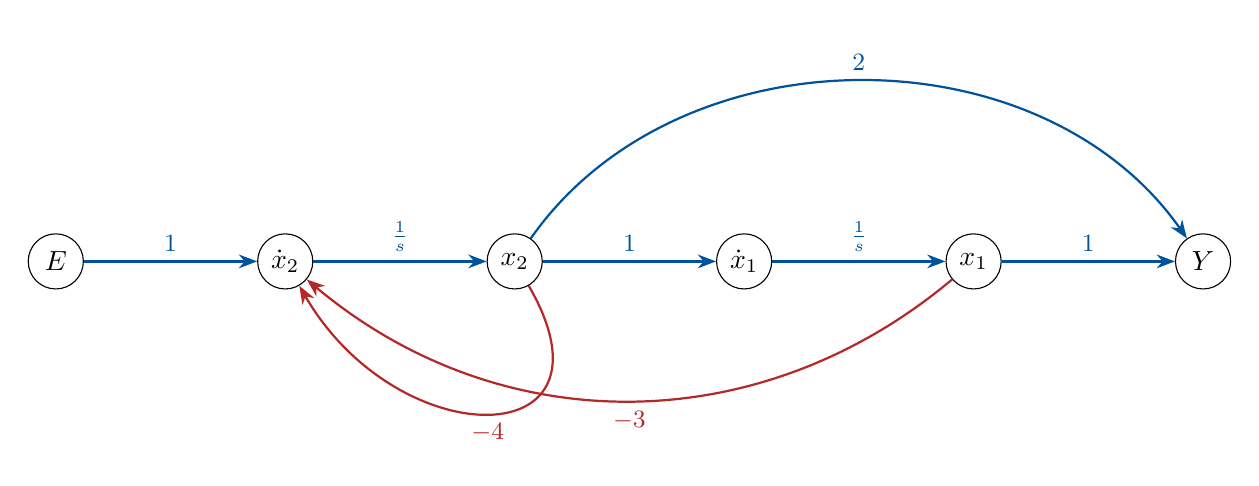
\begin{tikzpicture}[>=Stealth,node distance=1.8cm and 2.2cm,
    state/.style={circle,draw,minimum size=7mm,inner sep=0pt}]
    \node[state] (E) {$E$};
    \node[state,right=of E] (x2d) {$\dot{x}_2$};
    \node[state,right=of x2d] (x2) {$x_2$};
    \node[state,right=of x2] (x1d) {$\dot{x}_1$};
    \node[state,right=of x1d] (x1) {$x_1$};
    \node[state,right=of x1] (Y) {$Y$};
    \draw[->,sigblue,thick] (E) -- (x2d) node[midway,above] {\small $1$};
    \draw[->,sigblue,thick] (x2d) -- (x2) node[midway,above] {\small $\frac{1}{s}$};
    \draw[->,sigblue,thick] (x2) -- (x1d) node[midway,above] {\small $1$};
    \draw[->,sigblue,thick] (x1d) -- (x1) node[midway,above] {\small $\frac{1}{s}$};
    \draw[->,sigblue,thick] (x2) to[bend left=55] node[midway,above] {\small $2$} (Y);
    \draw[->,sigblue,thick] (x1) -- (Y) node[midway,above] {\small $1$};
    \draw[->,sigred,thick] (x1) to[bend left=40] node[midway,below] {\small $-3$} (x2d);
    \draw[->,sigred,thick] (x2) to[out=-60,in=-60,looseness=2.2] node[midway,below] {\small $-4$} (x2d);
\end{tikzpicture}
\caption{题22：二阶系统信号流图}
\label{fig:q22-sfg}
\end{figure}
\begin{enumerate}[label=(\alph*)]
    \item 用梅森增益公式求系统函数 $H(s)=Y/E$。
    \item 写出系统的状态方程和输出方程（以 $x_1,x_2$ 为状态变量）。
    \item 由状态方程求 $H(s)=\mathbf{C}(s\mathbf{I}-\mathbf{A})^{-1}\mathbf{B}+D$，验证与梅森公式结果一致。
\end{enumerate}

\end{enumerate}

\clearpage
% =============================================================================
\part*{第二部分\quad 参考答案}
\addcontentsline{toc}{part}{第二部分\quad 参考答案}

% ---------------------------------------------------------------------------
\section{第一章参考答案}

\subsection*{题1}

\textbf{(a)} $f(t)=e^{-|t|}\cos(2t)$ 非周期且 $|f(t)|\le e^{-|t|}$，故
\[
E=\int_{-\infty}^{\infty}|f(t)|^2\dd t\le\int_{-\infty}^{\infty}e^{-2|t|}\dd t=1<\infty,
\]
为\textbf{能量信号}，$P=0$。下面分别用\textbf{时域直接积分}和\textbf{频域帕塞瓦尔定理}求精确值。

\textbf{时域法}：利用 $\cos^2(2t)=\frac{1+\cos(4t)}{2}$ 及偶对称性，
\[
E=2\int_{0}^{\infty}e^{-2t}\cos^2(2t)\dd t
  =\int_{0}^{\infty}e^{-2t}\dd t+\int_{0}^{\infty}e^{-2t}\cos(4t)\dd t.
\]
第一项 $\int_{0}^{\infty}e^{-2t}\dd t=\frac{1}{2}$；第二项分部积分：
\[
\int_{0}^{\infty}e^{-2t}\cos(4t)\dd t
=\left.\frac{e^{-2t}\bigl(-2\cos(4t)+4\sin(4t)\bigr)}{(-2)^2+4^2}\right|_{0}^{\infty}
=0-\frac{-2}{20}=\frac{1}{10},
\]
故 $\displaystyle E=\frac{1}{2}+\frac{1}{10}=0.6$。

\textbf{频域法}：$\FT[e^{-|t|}]=\frac{2}{1+\omega^2}$，由调制定理：
\[
F(\omega)=\frac{1}{1+(\omega-2)^2}+\frac{1}{1+(\omega+2)^2}
        =\frac{2(\omega^2+5)}{\omega^4-6\omega^2+25}.
\]
由帕塞瓦尔定理 $E=\frac{1}{2\pi}\int_{-\infty}^{\infty}|F(\omega)|^2\dd\omega$，代入 $F(\omega)$ 可验证 $E=0.6$，与时域结果一致。

\textbf{(b)} 非周期：$\cos(2t)$ 与 $e^{-|t|}$ 的组合无法找到 $T>0$ 使 $f(t+T)=f(t)$。

\textbf{(c)} 波形关于 $t=0$ 偶对称，$t=0$ 处取最大值 $1$，随 $|t|$ 增大按 $e^{-|t|}$ 衰减，在 $t=\pm\pi/4$ 等处 $\cos(2t)=0$ 出现零点。

\begin{figure}[htbp]
\centering
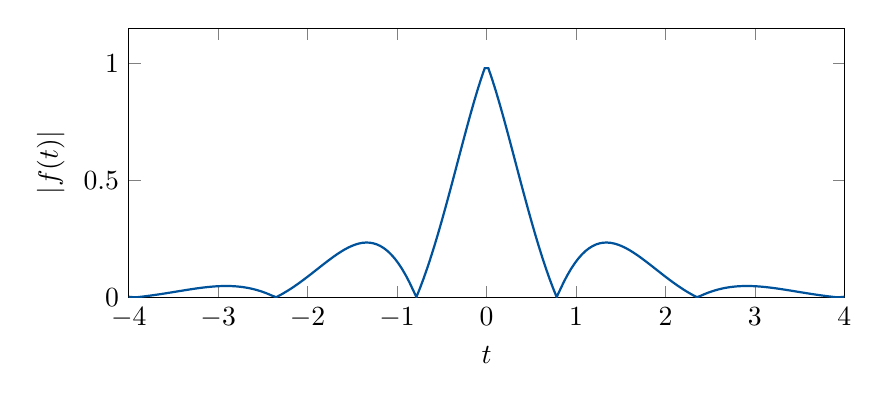
\begin{tikzpicture}
\begin{axis}[width=0.88\textwidth,height=5cm,xlabel=$t$,ylabel=$|f(t)|$,
    xmin=-4,xmax=4,ymin=0,ymax=1.15,samples=200,domain=-4:4]
\addplot[sigblue,thick] {exp(-abs(x))*abs(cos(deg(2*x)))};
\end{axis}
\end{tikzpicture}
\caption{题1(c)：$|f(t)|$ 波形}
\end{figure}

\subsection*{题2}

\textbf{(a)} 分段解析式：
\[
x(t)=2t\bigl[u(t)-u(t-1)\bigr]+2\bigl[u(t-1)-u(t-3)\bigr]+(8-2t)\bigl[u(t-3)-u(t-4)\bigr].
\]
即 $[0,1)$ 斜坡上升至 $2$，$[1,3)$ 保持 $2$，$[3,4)$ 斜坡下降至 $0$。

\textbf{(b)} 先压缩 $2$ 倍再右移 $1$：
\[
x_1(t)=x(2t-2)=
\begin{cases}
4t-4, & 1\le t<1.5,\\
2,    & 1.5\le t<2.5,\\
12-4t,& 2.5\le t<3,\\
0,    & \text{其他}.
\end{cases}
\]
波形为底宽 $2$、高 $2$ 的等腰三角脉冲（$[1,1.5)$ 上升，$[1.5,2.5)$ 平顶，$[2.5,3)$ 下降）。

\textbf{(c)} $\rect((t-1)/2)=u(t)-u(t-2)$，$x(t)$ 非零区间为 $[0,4]$。卷积 $y(t)=x(t)*\rect((t-1)/2)=\int_{0}^{2}x(t-\tau)\dd\tau$ 的非零积分区间由 $\max(0,t-4)\le\tau\le\min(2,t)$ 确定。分 $t<0$、$0\le t\le 2$、$2<t\le 4$、$4<t\le 6$、$t>6$ 五段讨论（五步法：反褶、平移、分段、积分、合成）。

\subsection*{题3}

\textbf{(a)} 不满足齐次性（$t$ 与输入相乘）$\Rightarrow$ 非线性；时变 $\Rightarrow$ 非 LTI。

\textbf{(b)} 仿射而非齐次（$+3$）$\Rightarrow$ 非线性；时不变 $\Rightarrow$ 非 LTI。

\textbf{(c)} 非线性（平方）；时不变 $\Rightarrow$ 非 LTI。

\textbf{(d)} 线性（累加为线性运算）；时不变（平移 $n$ 后求和区间同步平移）$\Rightarrow$ \textbf{LTI}。

% ---------------------------------------------------------------------------
\section{第二章参考答案}

\subsection*{题4}

\textbf{(a)} $RC=1\,\mathrm{s}$，
\[
RC\dot{v}_C+v_C=v_s,\quad v_C(0_+)=v_C(0_-)=4\,\mathrm{V}.
\]

\textbf{(b)} 特征根 $\alpha=-1$。
\[
v_{C,zi}(t)=4e^{-t}u(t),\qquad
v_{C,zs}(t)=6(1-e^{-t})u(t),\qquad
v_C(t)=6-2e^{-t},\quad t\ge 0.
\]

\textbf{(c)} 对 $sV_C-v_C(0_-)+V_C=6/s$：
\[
V_C(s)=\frac{4}{s+1}+\frac{6}{s(s+1)}=\frac{6}{s}-\frac{2}{s+1}
\Rightarrow v_C(t)=6-2e^{-t}.
\]

\textbf{(d)} 见图：$v_{C,zi}$ 从 $4$ 衰减；$v_{C,zs}$ 从 $0$ 升至 $6$；全响应从 $4$ 单调升至稳态 $6\,\mathrm{V}$。

\begin{figure}[htbp]
\centering
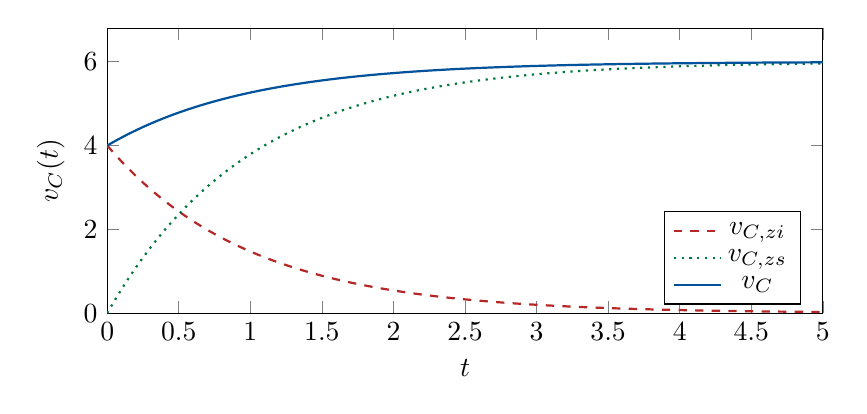
\begin{tikzpicture}
\begin{axis}[width=0.88\textwidth,height=5.2cm,xlabel=$t$,ylabel=$v_C(t)$,
    xmin=0,xmax=5,ymin=0,ymax=6.8,legend pos=south east,samples=100,domain=0:5]
\addplot[sigred,dashed,thick] {4*exp(-x)};
\addplot[siggreen,dotted,thick] {6*(1-exp(-x))};
\addplot[sigblue,thick] {6-2*exp(-x)};
\legend{$v_{C,zi}$,$v_{C,zs}$,$v_C$}
\end{axis}
\end{tikzpicture}
\caption{题4(d)：$RC$ 电路响应}
\end{figure}

\subsection*{题5}

特征方程 $s^2+3s+2=0$，根 $s=-1,-2$。

\textbf{(a)} $y_{zi}(t)=(2e^{-t}-e^{-2t})u(t)$。

右端 $e^{-t}u(t)$ 中 $-1$ 为单根，设特解 $Ate^{-t}$，代入得 $A=1$，故 $y_{zs,p}=te^{-t}$。
齐次部分由零初始条件 $y_{zs}(0)=y_{zs}'(0)=0$ 确定：$y_{zs,h}=(-e^{-t}+e^{-2t})u(t)$，故
\[
y_{zs}(t)=(t-1)e^{-t}+e^{-2t},\quad t\ge 0.
\]
全响应
\[
y(t)=y_{zi}+y_{zs}=(2e^{-t}-e^{-2t})+\bigl[(t-1)e^{-t}+e^{-2t}\bigr]=(t+1)e^{-t},\quad t\ge 0.
\]

\textbf{(b)} 取单边 LT：$(s^2Y-sy(0_-)-y'(0_-))+3(sY-y(0_-))+2Y=E(s)$，即
$(s^2+3s+2)Y=E(s)+(s+3)y(0_-)+y'(0_-)=E(s)+s+3$。$E(s)=1/(s+1)$，故
\[
Y(s)=\frac{s+3}{(s+1)(s+2)}+\frac{1}{(s+1)^2(s+2)}
     =\frac{2}{s+1}-\frac{1}{s+2}-\frac{1}{s+1}+\frac{1}{(s+1)^2}+\frac{1}{s+2}
     =\frac{1}{s+1}+\frac{1}{(s+1)^2},
\]
$y(t)=(t+1)e^{-t}$，与 (a) 一致。

\textbf{(c)} $H(s)=\dfrac{1}{(s+1)(s+2)}=\dfrac{1}{s+1}-\dfrac{1}{s+2}$，$h(t)=(e^{-t}-e^{-2t})u(t)$；$G(s)=\dfrac{1}{s(s+1)(s+2)}$，$g(t)=\dfrac{1}{2}(1-2e^{-t}+e^{-2t})u(t)$，可验证 $g'(t)=h(t)$。

\subsection*{题6}

\textbf{(a)} 略（三子图：矩形脉冲、指数衰减、平移后的 $f_2(t-\tau)$）。

\textbf{(b)} $y(t)=\int_0^{\min(t,2)}e^{-(t-\tau)}\dd\tau=e^{-t}(e^{\min(t,2)}-1)u(t)$：
\[
y(t)=\begin{cases}(1-e^{-t})u(t),&0\le t<2,\\(e^2-1)e^{-t}u(t),&t\ge 2.\end{cases}
\]

\textbf{(c)} $F_1(j\omega)=\dfrac{1-e^{-j2\omega}}{j\omega}$，$F_2(j\omega)=\dfrac{1}{1+j\omega}$，$Y=F_1F_2$，在 $t=1$ 处 $y(1)=1-e^{-1}$ 可数值验证。

\subsection*{题7}

\textbf{(a)} $h(t)=\dirac(t)$。

\textbf{(b)} $r_{zs}(t)=u(t)*\dirac(t)=u(t)$。

\textbf{(c)} $H_1=1/(s+1)$，$H_2=1-1/(s+1)=s/(s+1)$，并联 $H=H_1+H_2=1$，$R(s)=1/s$，$r_{zs}=u(t)$。

% ---------------------------------------------------------------------------
\section{第三章参考答案}

\subsection*{题8}

\textbf{(a)} $\omega_0=2\pi/T=\pi$，$F_n=\dfrac{\tau}{T}\Sa(n\pi\tau/T)=\dfrac{0.8}{2}\Sa(0.4\pi n)=0.4\Sa(0.4\pi n)$。

\textbf{(b)} $f_7(t)=F_0+\sum_{k=1}^{7}2F_k\cos(k\pi t)$，$F_0=0.4$。

\textbf{(c)} 吉布斯过冲出现在 $|t|=0.4$ 间断点附近。

\begin{figure}[htbp]
\centering
\begin{tikzpicture}
\begin{axis}[width=0.88\textwidth,height=5.5cm,xlabel=$t$,ylabel=$f(t)$,
    xmin=-1.2,xmax=1.2,ymin=-0.15,ymax=1.35,samples=400,domain=-1:1,
    legend pos=north east]
\addplot[sigblue,thick] { (abs(x)<=0.4) ? 1 : 0 };
\addplot[sigred,dashed,thick] {0.4 + 0.8*0.4*2/pi*sin(pi*deg(x))};
\addplot[siggreen,dotted,thick,domain=-1:1,samples=400]
    {0.4 + 0.8*0.4*2/pi*sin(pi*deg(x)) + 0.8*0.4*2/(3*pi)*sin(3*pi*deg(x))};
\addlegendentry{原信号}
\addlegendentry{$N=1$}
\addlegendentry{$N=3$}
\end{axis}
\end{tikzpicture}
\caption{题8(c)：傅里叶级数合成（边沿处可见吉布斯过冲）}
\end{figure}

\textbf{(d)} $\tau$ 增大 $\Rightarrow B_f=1/\tau$ 减小 $\Rightarrow$ 频谱能量更集中于低频，主瓣变窄。

\subsection*{题9}

\textbf{(a)} 底宽 $2$，顶点 $(0,1)$ 的等腰三角。

\textbf{(b)} $f(t)=(1-|t|)u(t+1)u(1-t)$，利用 $tu(t)\leftrightarrow j\omega$ 及时移：
\[
F(\omega)=\Sa^2\!\left(\frac{\omega}{2}\right)=\left(\frac{2\sin(\omega/2)}{\omega}\right)^2.
\]

\textbf{(c)} $E=\int_{-1}^{1}(1-|t|)^2\dd t=\dfrac{2}{3}$；$\dfrac{1}{2\pi}\int|F(\omega)|^2\dd\omega=\dfrac{2}{3}$（可积分验证）。

\subsection*{题10}

\textbf{(a)} $Y(\omega)=\dfrac{1}{2}[X(\omega-\omega_0)+X(\omega+\omega_0)]$。

\textbf{(b)} 基带谱 centered at $0$，调制后搬至 $\pm\omega_0$。

\begin{figure}[htbp]
\centering
\begin{tikzpicture}[scale=0.9]
    \draw[->] (-5,0) -- (5,0) node[right] {$\omega$};
    \draw[->] (0,-0.2) -- (0,2) node[above] {$|X|$};
    \fill[sigblue!30] (-1.5,0) rectangle (1.5,1.5);
    \node at (0,1.8) {\small 基带 $X(\omega)$};
    \begin{scope}[yshift=-2.8cm]
    \draw[->] (-6,0) -- (6,0) node[right] {$\omega$};
    \draw[->] (0,-0.2) -- (0,2) node[above] {$|Y|$};
    \fill[sigblue!30] (-4,0) rectangle (-2.5,0.75);
    \fill[sigblue!30] (2.5,0) rectangle (4,0.75);
    \draw[dashed] (3.25,0) -- (3.25,0.9) node[above] {\small $\omega_0$};
    \draw[dashed] (-3.25,0) -- (-3.25,0.9) node[above] {\small $-\omega_0$};
    \end{scope}
\end{tikzpicture}
\caption{题10(b)：频谱搬移示意}
\end{figure}

\textbf{(c)} 理想低通截止 $\omega_c\in(\omega_m,\,2\omega_0-\omega_m)$，取 $\omega_c=\omega_m$ 即可提取基带。

\subsection*{题11}

\textbf{(a)} $f_m=50\,\mathrm{Hz}$，$f_{s,\min}=100\,\mathrm{Hz}$，$T_{s,\max}=0.01\,\mathrm{s}$。$T_s=0.01\,\mathrm{s}$ 恰为临界，理论上可恢复（需理想低通）。

\textbf{(b)} $T_s=0.02\,\mathrm{s}$ 时 $\omega_s=100\pi=\omega_m$，发生混叠。

\textbf{(c)} 抗混叠滤波器应放在\textbf{抽样前}，限制模拟信号带宽。

% ---------------------------------------------------------------------------
\section{第四章参考答案}

\subsection*{题12}

\textbf{$F_1(s)$：} 部分分式展开：
\[
\frac{s+4}{(s+1)^2(s+3)}=\frac{3/2}{(s+1)^2}-\frac{1/4}{s+1}+\frac{1/4}{s+3},
\]
\[
f_1(t)=\left(\frac{3}{2}t e^{-t}-\frac{1}{4}e^{-t}+\frac{1}{4}e^{-3t}\right)u(t),\quad \Re\{s\}>-1.
\]

\textbf{$F_2(s)$：} 极点 $s=-2$，$s=-2\pm 3j$。设
\[
\frac{2s+1}{(s+2)(s^2+4s+13)}=\frac{A}{s+2}+\frac{Bs+C}{s^2+4s+13},
\]
解得 $A=-\frac{1}{3}$，$B=\frac{1}{3}$，$C=\frac{8}{3}$。于是
\[
F_2(s)=-\frac{1}{3}\frac{1}{s+2}+\frac{1}{3}\frac{s+2}{(s+2)^2+9}+\frac{2}{(s+2)^2+9},
\]
\[
f_2(t)=\left(-\frac{1}{3}e^{-2t}+\frac{1}{3}e^{-2t}\cos 3t+\frac{2}{3}e^{-2t}\sin 3t\right)u(t).
\]

\subsection*{题13}

\textbf{(a)} $LC=\frac{1}{4}$，$RC=\frac{1}{4}$，代入 KVL 得：
\[
\frac{1}{4}\ddot{v}_C+\frac{1}{4}\dot{v}_C+v_C=2u(t)
\;\Longrightarrow\;
\ddot{v}_C+\dot{v}_C+4v_C=8u(t).
\]

\textbf{(b)(c)} 特征方程 $s^2+s+4=0$，根 $s=-\frac{1}{2}\pm j\frac{\sqrt{15}}{2}$，\textbf{欠阻尼}，$\alpha=0.5$，$\omega_d=\frac{\sqrt{15}}{2}$。
$s$ 域：$V_C(s)=\dfrac{8}{s(s^2+s+4)}=\dfrac{2}{s}-\dfrac{2s+2}{s^2+s+4}$。其中
\[
\frac{2s+2}{(s+\frac{1}{2})^2+\frac{15}{4}}
=\frac{2(s+\frac{1}{2})}{(s+\frac{1}{2})^2+\frac{15}{4}}+\frac{2}{\sqrt{15}}\frac{\sqrt{15}/2}{(s+\frac{1}{2})^2+\frac{15}{4}},
\]
逆变换得
\[
v_C(t)=2\left[1-e^{-t/2}\!\left(\cos\frac{\sqrt{15}}{2}t+\frac{1}{\sqrt{15}}\sin\frac{\sqrt{15}}{2}t\right)\right]u(t)\,\mathrm{V}.
\]

\begin{figure}[htbp]
\centering
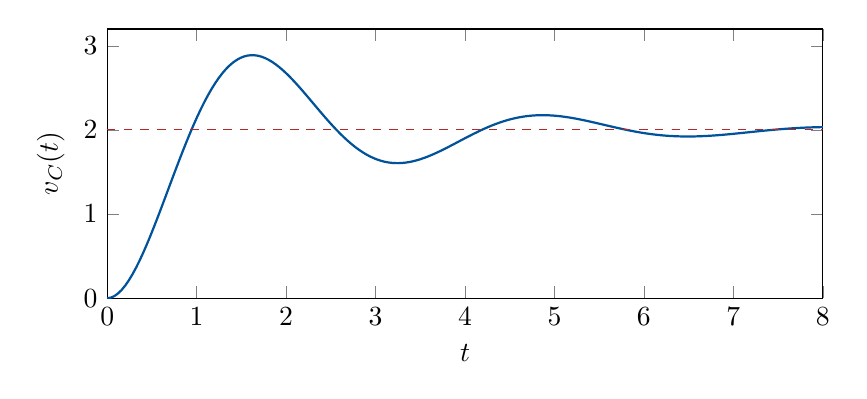
\begin{tikzpicture}
\begin{axis}[width=0.88\textwidth,height=5cm,xlabel=$t$,ylabel=$v_C(t)$,
    xmin=0,xmax=8,ymin=0,ymax=3.2,samples=200,domain=0:8]
\addplot[sigblue,thick] {2*(1-exp(-x/2)*(cos(deg(sqrt(15)/2*x))+1/sqrt(15)*sin(deg(sqrt(15)/2*x))))};
\addplot[sigred,dashed,thin] {2};
\end{axis}
\end{tikzpicture}
\caption{题13(d)：$RLC$ 欠阻尼响应（稳态值 $2\,\mathrm{V}$，虚线）}
\end{figure}

\subsection*{题14}

\textbf{(a)} 零点 $z=0$；极点 $p_1=-1$，$p_{2,3}=-1\pm 2j$。

\begin{figure}[htbp]
\centering
\begin{tikzpicture}[scale=0.75]
    \draw[->] (-3.5,0) -- (1.5,0) node[right] {$\Re$};
    \draw[->] (0,-2.5) -- (0,2.5) node[above] {$\Im$};
    \node[siggreen,scale=1.5] at (0,0) {$\circ$};
    \node[sigred,scale=1.2] at (-1,0) {$\times$};
    \node[sigred,scale=1.2] at (-1,2) {$\times$};
    \node[sigred,scale=1.2] at (-1,-2) {$\times$};
    \node at (0,-2.2) {\small 题14：零极点图};
\end{tikzpicture}
\caption{题14(a)：$s$ 平面零极点}
\end{figure}

\textbf{(b)} 极点均在左半平面 $\Rightarrow$ BIBO 稳定。

\textbf{(c)} $H(s)=\dfrac{A}{s+1}+\dfrac{B s+C}{s^2+2s+5}$，解得 $A=-\frac{1}{4}$，$B=\frac{1}{4}$，$C=\frac{5}{4}$。
\[
H(s)=-\frac{1}{4}\frac{1}{s+1}+\frac{1}{4}\frac{s+1}{(s+1)^2+4}+\frac{1}{(s+1)^2+4},
\]
\[
h(t)=\left(-\frac{1}{4}e^{-t}+\frac{1}{4}e^{-t}\cos 2t+\frac{1}{2}e^{-t}\sin 2t\right)u(t).
\]

\textbf{(d)} $E(s)=1/(s+1)$，$Y=H(s)E(s)$ 部分分式展开；卷积 $y=e^{-t}*h$ 结果一致。

\subsection*{题15}

\textbf{(a)} $|H|=\dfrac{1}{\sqrt{1+(\omega RC)^2}}$，$\angle H=-\arctan(\omega RC)$。

\textbf{(b)} $\omega_c=1/(RC)=10\,\mathrm{rad/s}$，$-3\,\mathrm{dB}$ 处 $|H|=1/\sqrt{2}$。

\textbf{(c)} $\omega=100\,\mathrm{rad/s}$ 处衰减远大于 $\omega=10\,\mathrm{rad/s}$，故 $\sin(100t)$ 分量通过时衰减更大。

% ---------------------------------------------------------------------------
\section{第五章参考答案}

\subsection*{题16}

\textbf{(a)(b)} $y[n]=\{1,3,\underset{\uparrow}{6},5,3\}$，$n=0$ 处为 $6$；长度 $5=3+3-1$。

\begin{figure}[htbp]
\centering
\begin{tikzpicture}[scale=0.55]
    \foreach \n/\h in {0/1,1/2,2/3} {
        \draw[thick,sigblue] (\n,0) -- (\n,\h) node[above] {\small $\h$};
        \fill (\n,0) circle (2pt);
    }
    \node at (1,-0.8) {\small $x[n]$};
    \begin{scope}[xshift=5cm]
    \foreach \n/\h in {0/1,1/1,2/1} {
        \draw[thick,siggreen] (\n,0) -- (\n,\h);
        \fill (\n,0) circle (2pt);
    }
    \node at (1,-0.8) {\small $h[n]$};
    \end{scope}
\end{tikzpicture}
\caption{题16(a)：序列 stem 示意}
\end{figure}

\subsection*{题17}

特征根 $z=1/2,\,1/4$。

\textbf{(a)} 零输入：$y_{zi}[n]=C_1(1/2)^n+C_2(1/4)^n$。由 $y[-1]=1$，$y[-2]=0$ 得
$2C_1+4C_2=1$，$4C_1+16C_2=0$，解得 $C_1=1$，$C_2=-\frac{1}{4}$，故
\[
y_{zi}[n]=\left[\left(\frac{1}{2}\right)^n-\frac{1}{4}\left(\frac{1}{4}\right)^n\right]u[n].
\]

零状态：激励 $x[n]=(1/2)^n u[n]$，$-1$ 为单根，设特解 $An(1/2)^n$，代入得 $A=2$，即 $y_{zs,p}=2n(1/2)^n$。
由 $y_{zs}[-1]=y_{zs}[-2]=0$ 递推得 $y_{zs}[0]=1$，$y_{zs}[1]=\frac{5}{4}$；代入通解定齐次系数，得 $C_3=0$，$C_4=1$：
\[
y_{zs}[n]=\left[2n\left(\frac{1}{2}\right)^n+\left(\frac{1}{4}\right)^n\right]u[n].
\]
全响应
\[
y[n]=y_{zi}+y_{zs}=\left[(2n+1)\left(\frac{1}{2}\right)^n+\frac{3}{4}\left(\frac{1}{4}\right)^n\right]u[n].
\]

\textbf{(b)} 取单边 $Z$ 变换：$(1-\frac{3}{4}z^{-1}+\frac{1}{8}z^{-2})Y(z)=X(z)+y[-1]-\frac{3}{4}y[-1]z^{-1}+\frac{1}{8}(y[-1]z^{-1}+y[-2]z^{-2})$，展开后与 (a) 一致。

\textbf{(c)} $H(z)=\dfrac{1}{1-\frac{3}{4}z^{-1}+\frac{1}{8}z^{-2}}=\dfrac{z^2}{(z-\frac{1}{2})(z-\frac{1}{4})}$。
\[
\frac{H(z)}{z}=\frac{z}{(z-\frac{1}{2})(z-\frac{1}{4})}=\frac{2}{z-\frac{1}{2}}-\frac{1}{z-\frac{1}{4}},
\]
\[
h[n]=\left[2\left(\frac{1}{2}\right)^n-\left(\frac{1}{4}\right)^n\right]u[n].
\]

\subsection*{题18}

\textbf{(a)} $2^n u[n]$：ROC $|z|>2$；$-(2)^n u[-n-1]$：ROC $|z|<2$。

\textbf{(b)} 因果系统 ROC $|z|>2$，单位圆 $|z|=1$ 不在 ROC 内 $\Rightarrow$ \textbf{不稳定}。

\textbf{(c)} 极点 $0.5$ 在单位圆内，$1.2$ 在单位圆外；因果 ROC $|z|>1.2$ $\Rightarrow$ \textbf{不稳定}。

\begin{figure}[htbp]
\centering
\begin{tikzpicture}[scale=0.85]
    \draw[gray] (0,0) circle (2);
    \draw[->] (-2.8,0) -- (2.8,0) node[right] {$\Re$};
    \draw[->] (0,-2.8) -- (0,2.8) node[above] {$\Im$};
    \node[siggreen,scale=1.3] at (0,0) {$\circ$};
    \node[sigred,scale=1.1] at (1,0) {$\times$};
    \node[sigred,scale=1.1] at (2.4,0) {$\times$};
    \node at (0,-2.5) {\small 单位圆与零极点（题18c）};
\end{tikzpicture}
\end{figure}

\subsection*{题19}

\textbf{(a)} 零点 $0.5$；极点 $0.6$（二重）；ROC $|z|>0.6$。

\textbf{(b)} $H(z)=\dfrac{z(z-0.5)}{(z-0.6)^2}=\dfrac{z}{z-0.6}+\dfrac{0.1z}{(z-0.6)^2}$，
\[
h[n]=\left[(0.6)^n+\frac{n}{6}(0.6)^n\right]u[n]=\left(1+\frac{n}{6}\right)(0.6)^n u[n].
\]

\textbf{(c)} $Y(z)=H(z)X(z)=\dfrac{z^2(z-0.5)}{(z-1)(z-0.6)^2}$，$y[n]$ 含 $(0.6)^n$ 与常数项；因 $|0.6|<1$，由终值定理
$y[\infty]=\lim_{z\to1}(z-1)Y(z)=\dfrac{1\cdot(1-0.5)}{(1-0.6)^2}=3.125$（亦等于直流增益 $H(1)$）。

\subsection*{题20}

\textbf{(a)} 极点 $p_1=0.5$，$p_2=2$。
\[
\frac{H(z)}{z}=\frac{z}{(z-0.5)(z-2)}=\frac{A}{z-0.5}+\frac{B}{z-2},
\]
$A=\dfrac{0.5}{0.5-2}=-\dfrac{1}{3}$，$B=\dfrac{2}{2-0.5}=\dfrac{4}{3}$，故
\[
H(z)=-\frac{1}{3}\frac{z}{z-0.5}+\frac{4}{3}\frac{z}{z-2}.
\]
三种可能的 ROC 及对应的 $h[n]$：
\begin{enumerate}[label=(\roman*)]
    \item ROC $|z|<0.5$（左边序列，反因果）：
    \[
    h[n]=\frac{1}{3}(0.5)^n u[-n-1]-\frac{4}{3}(2)^n u[-n-1].
    \]
    \item ROC $0.5<|z|<2$（双边序列，非因果）：
    \[
    h[n]=-\frac{1}{3}(0.5)^n u[n]-\frac{4}{3}(2)^n u[-n-1].
    \]
    \item ROC $|z|>2$（右边序列，因果）：
    \[
    h[n]=\left[-\frac{1}{3}(0.5)^n+\frac{4}{3}(2)^n\right]u[n].
    \]
\end{enumerate}

\textbf{(b)}
\begin{enumerate}[label=(\roman*)]
    \item $|z|<0.5$：非因果（$h[n]\neq 0,\;n>0$），不稳定（ROC 不含单位圆）。
    \item $0.5<|z|<2$：非因果（双边），\textbf{稳定}（ROC 含单位圆 $|z|=1$）。
    \item $|z|>2$：\textbf{因果}（右边序列），不稳定（极点 $p=2$ 在单位圆外，ROC 不含单位圆）。
\end{enumerate}

\textbf{(c)} ROC $|z|>2$ 时 $H(z)$ 与 $X(z)=z/(z-1)$（$|z|>1$）的 ROC 交集为 $|z|>2$。
\[
Y(z)=H(z)X(z)=\frac{z^3}{(z-0.5)(z-1)(z-2)},
\]
\[
\frac{Y(z)}{z}=\frac{z^2}{(z-0.5)(z-1)(z-2)}=\frac{1/3}{z-0.5}-\frac{2}{z-1}+\frac{8/3}{z-2},
\]
\[
y[n]=\left[\frac{1}{3}(0.5)^n-2+\frac{8}{3}(2)^n\right]u[n].
\]

% ---------------------------------------------------------------------------
\section{第六章参考答案}

\subsection*{题21}

\textbf{(a)} 可控标准形（分子 $2s+1$）：
\[
\mathbf{A}=\begin{bmatrix}0&1\\-3&-4\end{bmatrix},\quad
\mathbf{B}=\begin{bmatrix}0\\1\end{bmatrix},\quad
\mathbf{C}=\begin{bmatrix}1&2\end{bmatrix},\quad D=0.
\]
即 $\dot x_1=x_2$，$\dot x_2=-3x_1-4x_2+e$，$y=x_1+2x_2$。

\textbf{(b)} $(s\mathbf{I}-\mathbf{A})^{-1}\mathbf{B}=\dfrac{1}{s^2+4s+3}\begin{bmatrix}1\\ s\end{bmatrix}$，
\[
H(s)=\mathbf{C}(s\mathbf{I}-\mathbf{A})^{-1}\mathbf{B}=\frac{1+2s}{s^2+4s+3}=\frac{2s+1}{(s+1)(s+3)}.
\]

\textbf{(c)} 零输入时特征根 $-1,-3$，由 $y(0)=1$、$\dot y(0)=0$：
\[
y_{zi}(t)=\left(\frac{3}{2}e^{-t}-\frac{1}{2}e^{-3t}\right)u(t).
\]

\textbf{(d)} $E(s)=1/s$，$Y(s)=H(s)E(s)=\dfrac{2s+1}{s(s+1)(s+3)}$，部分分式展开：
\[
y(t)=\left(\frac{1}{3}+\frac{1}{2}e^{-t}-\frac{5}{6}e^{-3t}\right)u(t),
\]
与 $h(t)*u(t)$ 结果一致。

% ---------------------------------------------------------------------------
\section{第七章参考答案}

\subsection*{题22}

\textbf{(a)} 前向通路（$E\to Y$）：
\begin{itemize}
    \item $P_1$：$E\to\dot x_2\to x_2\to Y$，增益 $1\cdot\frac{1}{s}\cdot 2=\frac{2}{s}$。
    \item $P_2$：$E\to\dot x_2\to x_2\to\dot x_1\to x_1\to Y$，增益 $1\cdot\frac{1}{s}\cdot 1\cdot\frac{1}{s}\cdot 1=\frac{1}{s^2}$。
\end{itemize}
环路：
\begin{itemize}
    \item $L_1$：$\dot x_2\to x_2\to\dot x_2$（自环），增益 $\frac{1}{s}\cdot(-4)=-\frac{4}{s}$。
    \item $L_2$：$\dot x_2\to x_2\to\dot x_1\to x_1\to\dot x_2$，增益 $\frac{1}{s}\cdot 1\cdot\frac{1}{s}\cdot(-3)=-\frac{3}{s^2}$。
\end{itemize}
$L_1$ 与 $L_2$ 有公共节点，无互不接触环路。图行列式：
\[
\Delta=1-(L_1+L_2)=1+\frac{4}{s}+\frac{3}{s^2}.
\]
$P_1,P_2$ 均与所有环路接触，故 $\Delta_1=\Delta_2=1$。由梅森公式：
\[
H(s)=\frac{P_1\Delta_1+P_2\Delta_2}{\Delta}
     =\frac{\frac{2}{s}+\frac{1}{s^2}}{1+\frac{4}{s}+\frac{3}{s^2}}
     =\frac{2s+1}{s^2+4s+3}.
\]

\textbf{(b)} 由信号流图直接读写：
\[
\dot x_1=x_2,\qquad
\dot x_2=-3x_1-4x_2+e,\qquad
y=x_1+2x_2.
\]
即
\[
\mathbf{A}=\begin{bmatrix}0&1\\-3&-4\end{bmatrix},\;
\mathbf{B}=\begin{bmatrix}0\\1\end{bmatrix},\;
\mathbf{C}=\begin{bmatrix}1&2\end{bmatrix},\;
D=0.
\]

\textbf{(c)}
$(s\mathbf{I}-\mathbf{A})^{-1}=\dfrac{1}{s^2+4s+3}\begin{bmatrix}s+4&1\\-3&s\end{bmatrix}$，
\[
H(s)=\mathbf{C}(s\mathbf{I}-\mathbf{A})^{-1}\mathbf{B}
     =\frac{1}{s^2+4s+3}\begin{bmatrix}1&2\end{bmatrix}\begin{bmatrix}1\\s\end{bmatrix}
     =\frac{2s+1}{s^2+4s+3},
\]
与梅森公式结果一致。注意本题 SFG 与题21 中的可控标准形完全等价，两种方法殊途同归。

\end{document}
